\chapter{Калькулятор с выбором операции}

Калькулятор, который мы собирали раньше, поддерживал $7$~операций:
\begin{enumerate}
    \item Инверсия
    \item Сдвиг вправо
    \item Побитовое И
    \item Побитовое ИЛИ
    \item Исключающее ИЛИ
    \item Сложение
    \item Вычитание
\end{enumerate}

Однако у каждой операции был собственный набор переключателей-операндов.
А для логических операций ещё нужно было выбрать нужный выход.

Было бы удобнее отдельно вводить значения операндов, а лишь потом указывать
выполняемую операцию.

В итоге для каждого вычисления нужна следующая последовательность действий:
\begin{enumerate}
    \item Набрать значение первого операнда.
    \item Набрать значение второго операнда (если нужна бинарная операция).
    \item Выбрать выполняемую операцию.
    \item Загрузить получившийся результат в регистр.
\end{enumerate}

\section{Практикум}

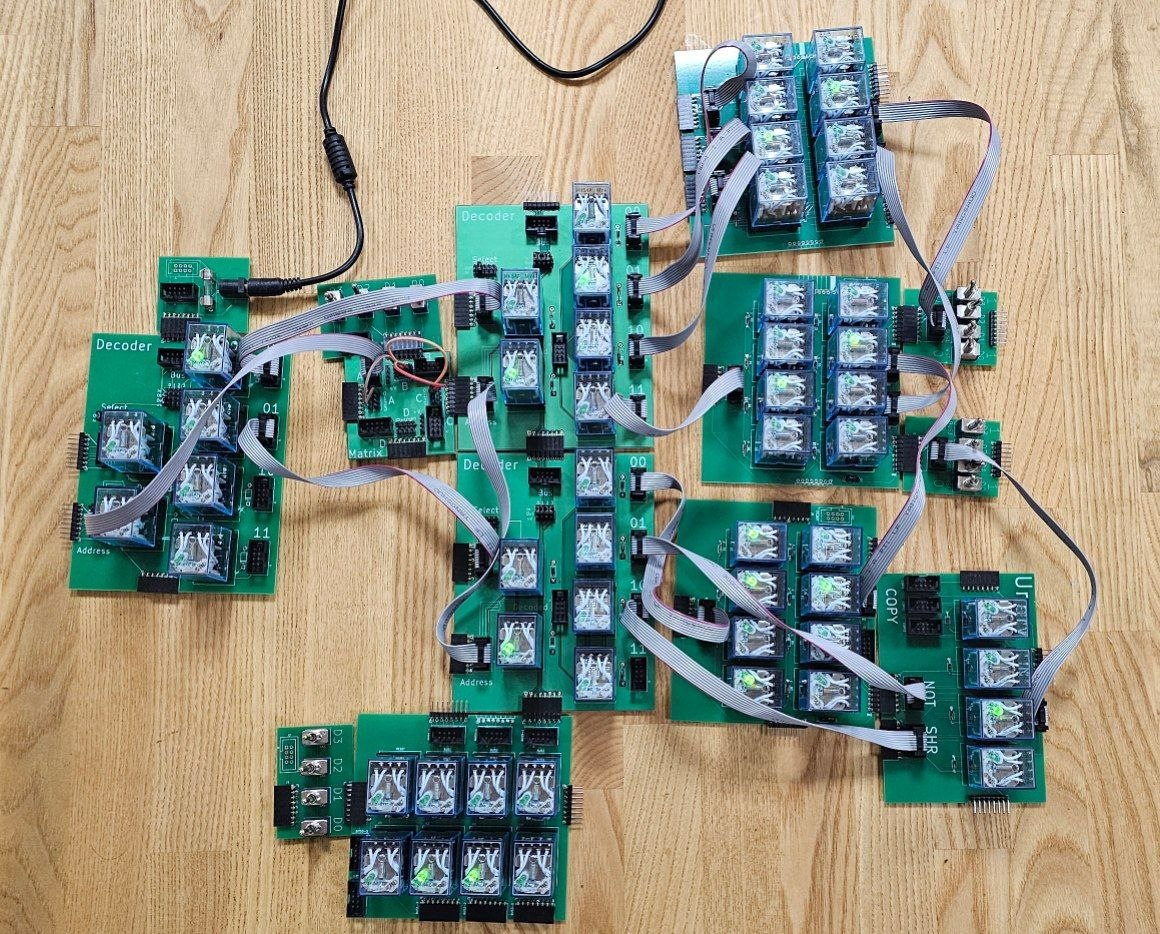
\includegraphics[width=\columnwidth]{photo/calculator2.jpg}

Можно сделать два варианта вычитания: с использованием отдельного инвертора
или с использованием инвертора, который делает унарные операции.
Во втором случае унарные операции будут работать со вторым операндом, а не
с первым.

Список модулей:
\begin{itemize}
    \item Модуль переключателей: $4$ штуки
    \item Модуль унарных операций: $1$ штука (или $2$ штуки)
    \item Сумматор: $2$ штуки
    \item Модуль логических операций: $1$ штука
    \item Дешифратор: $3$ штуки
    \item Регистровый модуль: $1$ штука
    \item Кросс-модуль: $1$ штука
\end{itemize}

